\documentclass[class=jsarticle, crop=false, dvipdfmx, fleqn]{standalone}
%% preamble for Numerical-structure-analysis report

\input{/Users/User/Documents/Project/TeX/preamble/mypreamble}

%% titles
\title{統計的機械学習 レポート}
\author{37-196360 \quad 森田涼介}


%% setting for listings
\newtcbinputlisting[auto counter]{\reportlisting}[3][]{%
	listing file = {#3},
	listing options = {language=python, style=tcblatex, numbers=left, numberstyle=\tiny},
	listing only,
	breakable,
	toprule at break = 0mm,
	bottomrule at break = 0mm,
	left = 6mm,
	sharp corners,
	drop shadow,
	title = Listings \thetcbcounter : \texttt{#2},
	label = #1,
	}



%% title format
\usepackage{titlesec}
\titleformat{\section}{\LARGE}{宿題\thesection}{0zw}{}
\newcommand{\sectionbreak}{\clearpage}
\titleformat{\subsection}{\Large}{\Alph{subsection})}{0zw}{}

\begin{document}
\section{}

ガウス混合モデルのEMアルゴリズムを実装し,
適当な一次元の確率密度関数を推定する。

今回は,
平均0・分散1の正規分布からのサンプリングのうち,
7割に2を足し,3割に\(-2\)を足した分布を用いる。
サンプル数\num{1000}点,および\num{10000}点について実験を行った。
この分布のサンプル数\num{1000}のときのヒストグラムを図\ref{fig:sample_hist}に示す。
なお,このヒストグラムは正規化されていることに注意されたい。

\begin{figure}[H]
    \centering
    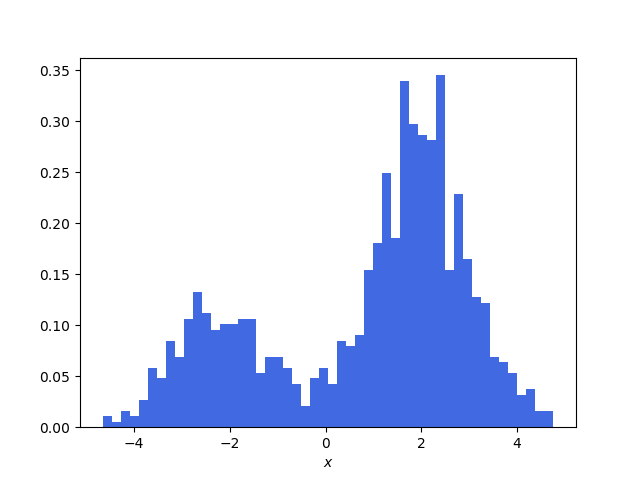
\includegraphics[clip, width=12cm]{../figures/assignment2_sample}
    \caption{実データのヒストグラム(サンプル数\num{1000})}
    \label{fig:sample_hist}
\end{figure}

パラメータの初期化は一様分布により行った。
\(w_j\)は総和が1となるようにし,
\(\bm{\mu}\)は\([-1.5,\ 1.5)\),
\(\sigma\)は\([0,\ 1)\)の一様分布を用いた。
また,実データを見ると,
2つの正規分布で近似するのが妥当だと考られるため,
\(m = 2\)とした。

結果は図\ref{fig:result_n1000},\ref{fig:result_n10000}に示した。
また,収束時のパラメータを表\ref{tab:result}に示す。
データの作り方から考えて,
平均2・分散1の正規分布と
平均\(-2\)・分散1の正規分布が
\(7:3\)で重ね合わせられている分布が真の分布であると考えられる。
表\ref{tab:result}を見ると,
特に\num{10000}点の場合は,
実際そのようなパラメータに近くなっていることがわかる。

\begin{figure}
    \centering
    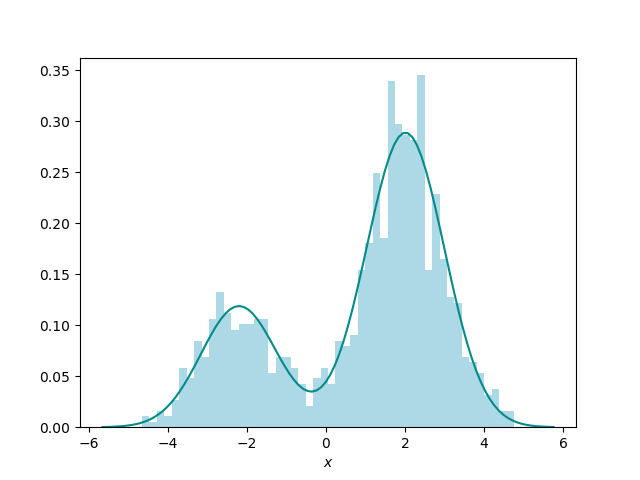
\includegraphics[clip, width=12cm]{../figures/assignment2_result_n1000}
    \caption{サンプル数\num{1000}のときの実データのヒストグラムとガウス混合モデル}
    \label{fig:result_n1000}
\end{figure}

\begin{figure}
    \centering
    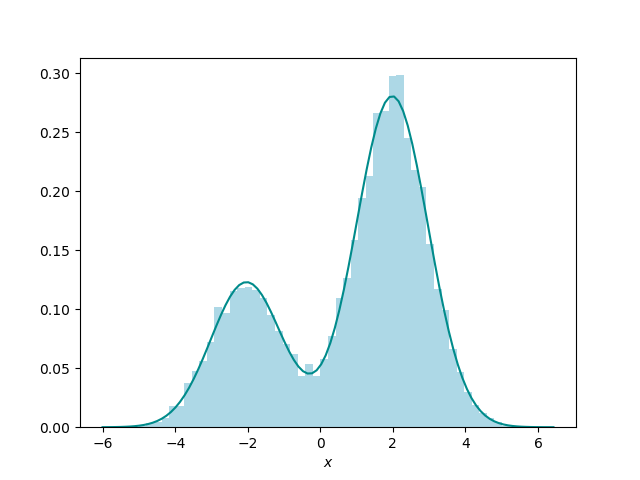
\includegraphics[clip, width=12cm]{../figures/assignment2_result_n10000}
    \caption{サンプル数\num{10000}のときの実データのヒストグラムとガウス混合モデル}
    \label{fig:result_n10000}
\end{figure}

\vspace*{3\baselineskip}

\begin{table}
    \centering
    \caption{収束時のパラメータと\(Q\)の値}
    \begin{tabular}{ccccccccc}
        \(n\) & \(Q\) & \(Q/n\) & \(w_1\) & \(w_2\) & \(\mu_1\) & \(\mu_2\) & \(\sigma_1\) & \(\sigma_2\) \\ \hline
        \num{1000} & \(-\num{1996}\) & \(-1.996\) & 0.7138 & 0.2862 & 2.013 & -2.201 & 0.9054 & 0.9614 \\
        \num{10000} & \(-\num{20194}\) & \(-2.019\) & 0.3020 & 0.6980 & \(-2.041\) & 1.980 & 0.9797 & 0.9916
    \end{tabular}
    \label{tab:result}
\end{table}


\end{document}
